\usepackage[scientific-notation=true]{siunitx}
\usepackage{float, verbatim, amsmath, amssymb, fullpage, paralist, cancel, listings, subfig, enumitem, siunitx, graphicx, xcolor, tikz, booktabs, tcolorbox, textcomp, url, parse lines, fontawesome5, marginnote, smartdiagram, forest, pifont, pgfcalendar, pgfgantt, fix-cm, ulem, soul, multirow, xfrac, colortbl, xspace, fontenc, helvet, mathptmx,ragged2e,csquotes} 
\definecolor{smcolor}{rgb}{0.8,0.5,0.5}
\definecolor{bsmcolor}{rgb}{0.4,0.6,0.8}
\definecolor{pvcolor}{rgb}{0.8,0.8,0.8}
\definecolor{cobalt}{rgb}{0.0, 0.28, 0.67}
\definecolor{darkelectricblue}{rgb}{0.33, 0.41, 0.47}
\definecolor{darkpowderblue}{rgb}{0.0, 0.2, 0.6}
\definecolor{darktangerine}{rgb}{1.0, 0.66, 0.07}
\definecolor{pastelviolet}{rgb}{0.8, 0.6, 0.79}
\definecolor{black}   {RGB}{0.0, 0.13, 0.28}
\definecolor{dukeblue}    {rgb}{0.0, 0.0, 0.61}
\definecolor{oxfordblue}{rgb}{0.0, 0.13, 0.28}
\definecolor{navyblue}{rgb}{0.0, 0.0, 0.5}
\definecolor{linkred}{RGB}{165,0,33}
\newcommand{\ccell}{\cellcolor{navyblue}}
\usesmartdiagramlibrary{additions}
\usepackage{hyperref}
\usepackage{cleveref}[capital]
\usepackage{textcase}
%\NoAutoCase 
\hypersetup{
        linktocpage=true,
        setpagesize=true,
	colorlinks= true,
	linkcolor=cobalt!50!black,
        menucolor=cobalt!50!black,
	filecolor=cobalt!50!black,      
	urlcolor=cobalt!50!black,
        citecolor=cobalt!50!black,
        citebordercolor=cobalt!50!black,
	pdftitle={Light Dark Scalar},
        pdfsubject={Latex},
        pdfauthor={Yoxara Villamizar},
        pdfkeywords={BSM Phenomenology, SM, Collider, DM}
}
\graphicspath{{Figures/}} 
%#######################ITEMIZES#################
\newenvironment{menumerate}{\begin{enumerate}[label=\textcolor{cobalt}\large{\textbf{\ding{\numexpr171+\value{enumi}}}\normalsize}] }{\end{enumerate}}%171, 181, 191, 201
\newlist{firstitemize}{itemize}{1}
\setlist[firstitemize,1]{label=\color{cobalt!70!black} \ding{111}, nosep, leftmargin=*, before=\normalcolor}
\newlist{seconditemize}{itemize}{1}
\setlist[seconditemize,1]{label=\color{cobalt!70!black}\ding{226}\normalcolor, nosep, leftmargin=*} %254
\newlist{thirditemize}{itemize}{1}
\setlist[thirditemize,1]{label=\color{cobalt!70!black} \ding{118}, nosep, leftmargin=*, before=\normalcolor}
%################################################
%################################################
\newcommand{\yox}[1]{{\color{magenta}#1}}
\newcommand{\zp}{\mathrm{Z}^{\prime}}
\newcommand{\mzpr}{\mathrm{m}_{\mathrm{Z}^{\prime}}}
\newcommand{\z}{\mathrm{Z}}
\newcommand{\w}{\mathrm{W}}
\newcommand{\zpm}{\mathrm{Z}^{\prime \mu}}
\newcommand{\nn}{\nonumber}
\newcommand{\up}{\mathrm{U(1)}^{\prime}}
\renewcommand{\bar}{\overline}
\newcommand{\lum}{\mathcal{L}}
\newcommand{\fb}{\mathrm{fb}}
\newcommand{\pb}{\mathrm{pb}}
\newcommand{\pt}{\bf \mathrm{p}_\mathrm{T}}
\newcommand{\ptj}{\bf \mathrm{p}_\mathrm{T (\mathrm{j_{1}})}}
\newcommand{\ptm}{\bf \overrightarrow{\mathrm{p}}_\mathrm{T}^{\mathrm{miss}}}
\newcommand{\ptv}{\bf \overrightarrow{\mathrm{p}}_\mathrm{T}}
\newcommand{\etm}{\mathrm{E}_\mathrm{T}^{\mathrm{miss}}}
\newcommand{\Ht}{\bf \mathrm{H}_\mathrm{T}}
\newcommand{\gev}{\mathrm{\, GeV}}
\newcommand{\tev}{\mathrm{\, TeV}}
\newcommand{\ga}{\bf \gamma}
\newcommand{\x}{\bf \chi}
\newcommand{\gq}{\mathrm{g}_{q}}
\newcommand{\gx}{\mathrm{g}_{\chi}}
\newcommand{\mx}{\mathrm{m}_{\chi}}
\newcommand{\mxx}{\mathrm{m}_{\chi \chi}}
\newcommand{\Em}{\mathrm{E}_\mathrm{T}^{\mathrm{miss}}}
\newcommand{\sUL}{\sigma_{\mathrm{UL}}}
\newcommand{\sTh}{\sigma_{\mathrm{The}}}
\usepackage{tikz}
\usetikzlibrary{arrows.meta,decorations,calc,shadows.blur,decorations.pathreplacing,decorations.pathmorphing,decorations.markings,shapes, arrows, positioning,bending,chains,matrix, patterns,mindmap,trees}
\tikzset{
>=triangle 45,
scalar/.style={decorate, dashed, draw=cobalt!50!black, thick, line width=0.8pt}, 
photon/.style={decorate, line width=0.85pt, draw=black, decoration={snake, segment length=5, amplitude=3pt, post length=0.5mm, pre length=0.5mm}}, 
particle/.style={draw=black, postaction={decorate}},
fermion/.style={draw=black, line width=0.6pt, postaction={decorate}, decoration={markings,mark=at position .5 with {\arrow[draw=black,scale=1.2,>=stealth]{>}}}},
antifermion/.style={draw=black, line width=0.6pt, postaction={decorate},decoration={markings,mark=at position .5 with {\arrow[draw=black,scale=1.2,>=stealth]{<}}}},
}

\newcommand\eetottP{
\resizebox{\linewidth}{!}{
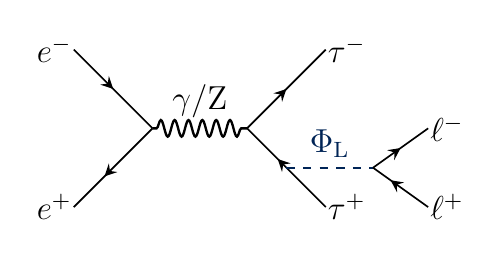
\begin{tikzpicture}
    % Incoming electron and positron
    \draw[fermion] (0,2.5) -- (1,1.5) node[at start, left, xshift=0.1cm] {\large $e^{-}$};
    \draw[antifermion] (0,0.5) -- (1,1.5) node[at start, left, xshift=0.1cm] {\large $e^{+}$};
    % Photon or Z
    \draw[photon] (1,1.5) -- (2.2,1.5) node[midway, above, yshift=-0.00cm] {\large $\gamma/\z$};
    % Outgoing tau particles
    \draw[fermion] (2.2,1.5) -- (3.2,2.5) node[at end, right, xshift=-0.1cm] {\large $\tau^{-}$};
    \draw[antifermion] (2.2,1.5) -- (3.2,0.5) node[at end, right, xshift=-0.1cm] { \large $\tau^{+}$};
    % Scalar particle interaction
    \draw[scalar] (2.7,1) -- (3.8,1) node[midway, above, yshift=-0.0cm, cobalt!50!black] { \large $\Phi_{\mathrm{L}}$};
    % Outgoing lepton pair
    \draw[fermion] (3.8,1) -- (4.5,1.5) node[at end, right, xshift=-0.1cm] {\large  $\ell^{-}$};
    \draw[antifermion] (3.8,1) -- (4.5,0.5) node[at end, right, xshift=-0.1cm] { \large $\ell^{+}$};
\end{tikzpicture}
}
}
